% !Mode:: "TeX:UTF-8"

\chapter{绪论}
随着互联网的蓬勃发展,复杂网络分析在实际应用特别是风险计算中的地位越来越高。尤其是动态网络的相关算法如动态网络社团检测,对于检测时序关联性数据即动态网络数据中突发事件的作用非常大。本章将会介绍动态复杂网络社团检测以及社团演化的研究背景及意义以及风险计算的研究背景、应用场景等。

\section{研究背景及意义}
随着以互联网为代表的网络信息技术的迅速发展,复杂网络对人类社会的影响越来越大。从万维网到社交网络,从病毒传播到交通流的管控分析,都能够从中提取出复杂网络结构~\cite{ben2004complex},进而通过对相应复杂网络的分析来获得现实网络的信息,进而达到改善用户体验、遏制病毒传播以及减少交通拥堵等目的。

复杂网络分析(complex network analysis)来源于图论,至今已有超过200年的历史,然而自从1998年nature上提出了复杂网络的“小世界”~\cite{watts1998collective}属性以及1999年science上提出了复杂网络的“无标度”~\cite{barabasi1999emergence}属性后,复杂网络分析才进入了飞速发展的时期。

作为复杂网络分析的重要任务之一,社团检测始终吸引了大量科研人员的注意力~\cite{rossetti2018community}。社团最广泛的定义就是----其作为网络中的子图,子图内部的节点连边密度多于子图与子图外其他节点的连边密度。例如,在万维网中,某个局域网内的服务器或pc之间基本是全连通的,而改局域网与外部仅仅通过一个路由器进行数据交换;再比如社交网络中的社团则代表了某个小团体,比如某兴趣团体等;而对于论文引用网络来说,社团结构则可以代表不同的研究领域等。社团检测则利用不同的理论去对网络中的节点进行聚类,以高效准确的找出不同网络中的社团结构。在现实世界中,人们往往利用动态网络对现实世界数据进行建模,并利用动态复杂网络分析的相关方法,对其进行分析。其中动态社团检测就是动态网络分析的重要的任务之一,而动态社团检测涉及两个主要任务,每个时间快照上的社团检测以及连续时间快照的社团演化分析。

动态社团检测能够帮助风险计算如城市风险事件的相关人员以及事件规模进行检测,而社团演化应用在风险计算如城市风险计算中所对应的就是风险事件的发生发展以及结束的整个过程的演化行为的计算。利用复杂网络建模,对城市多维动态数据进行合理的融合,再利用动态社团检测方法对风险事件进行计算以及对其发生发展进行合理推理,进而可以帮助人们把控风险因素以及风险事件。

\section{研究现状}
\subsection{复杂网络社团检测现状}

目前已经有大量的研究和方法聚焦于复杂网络社团检测任务,例如基于模块度的方法~\cite{waltman2013smart}、基于谱聚类的方法~\cite{krzakala2013spectral}以及生成模型~\cite{holland1976local}。在生成模型中,应用最广泛且发展最迅速的模型之一就是随机块模型(Stochastic Block Model)。随机块模型提出三个假设:(1)网络中每个节点属于一个社团;(2)网络中的两个节点之间有没有边只与节点所在的社团有关。(3)网络中的社团个数固定。经过多年的改进,随机块模型已经被应用在多个领域,例如生物信息学和社会科学等~\cite{airoldi2006mixed,hoff2002latent}。研究者对随机块模型进行了不同方向的扩展,例如Pal~\cite{pal2019scalable}等人提出了混合随机块模型,为每个节点分配了一个长度为社团个数的向量来衡量每个节点属于每个社团的概率或称为隶属度,从而使每个节点可以属于多个社团;Kemp~\cite{kemp2004discovering}等人提出了随机块模型的改进版模型,该模型允许网络可以存在无限数量的社团;而Hofman~\cite{hofman2008bayesian}等人则利用贝叶斯推断来推测随机块模型的最优解以及最优社团个数;Chen, Yudong~\cite{chen2018convexified}等人利用了节点的度来修正不同社团节点之间连边的概率,进而来修正随机块模型社团内部节点都是等价的这种不合理假设;类似的,Qiao, Maoying~\cite{qiao2018adapting}等人也引入了度衰减参数来修正这种不合理假设,同时还使得社团内部的节点在该模型中服从power law。

然而上述模型以及方法均面向的是静态网络,也就是网络中的节点与边不具有时间属性,不随时间变化。而真实世界的网络往往是动态的。动态网络社团检测的研究,也是近几年研究者们所重点关注的。动态网络的数据不同于静态网络,其数据引入了时间属性。同时动态网络的数据也具有不同的格式,对于动态网络数据有两种数据格式,第一种是将连续时间的网络数据切分成等时间间隔的静态网络再进行处理;第二种是将网络数据写成三元组的形式,即{源点,汇点,持续时间}来表示一条边的生命周期。第一种形式便于处理,且可以有效利用静态网络的算法拓展到动态网络中,这种格式数据的缺陷是对于相邻网络切片的时间间隔不好把控;而第二种形式相比于第一种形式更加连续,更能保持动态网络的变化,然而这种格式的数据不易于处理,并且较难借鉴静态网络算法。综合考虑,我们的工作主要针对第一种数据格式,即对网络进行切片处理后进行数据分析。
对于动态网络社团检测任务,主要包括两方面,第一方面是每个时间片的社团检测;第二个方面是不同时间片的社团演化\cite{rossetti2018community,dakiche2019tracking}。动态网络社团检测的方法多种多样,包括两步法、进化聚类法以及生成模型等。两步法就是对于每个时间片运行静态网络社团检测的算法,然后再在相邻时间片进行社团匹配~\cite{tajeuna2015tracking}。这种方法完全割裂了社团检测和社团演化,对于网络噪声非常敏感,因此在真实网络中效果不好。进化聚类认为当前时间的网络社团结构与前一个时间片或者前几个时间片的社团有关,因此在计算当前时间片的社团结构时,进化聚类会将上一个时间片的社团检测结果输入到算法中来提高社团检测效果~\cite{jiang2019efficient}。而生成模型则认为当前时刻的社团结构是由一个特定的与整个网络有关的分布生成的,因此生成模型会利用已知信息对网络进行建模,通过对模型的推断求解得出当前所有时间片的社团结构~\cite{yang2011detecting}。

Yang等人~\cite{yang2011detecting}在2011年将随机块模型应用到动态网络中,提出了DSBM即动态随机块模型。该模型引入了节点的社团转移矩阵,通过该矩阵来把握社团的演化行为,并通过采样对模型进行求解。该方法初步将社团检测和社团演化融合到了一起,但是对于社团演化的把握粒度较粗,同时依然需要提前确定社团个数并且不能处理重叠社团问题,并且其依然遵循社团内部节点地位等同的假设。Tang, Xuning~\cite{tang2011dynamic}提出了DBTDP,利用狄利克雷过程进行模型选择,从而解决了社团个数必须提前确定的不合理假设。而Wu,xunxun~\cite{wu2019dynamic}等人将节点的度衰减参数引入了动态网络,并利用变分推断对模型进行求解,使得模型的节点度符合真实网络的power law。Kao, Edward K~\cite{kao2018hybrid}等人将混合随机块模型拓展到了动态网络,打破了动态随机块模型中每个几点只能属于一个社团的假设。
\begin{figure}[htbp]
	\centering
	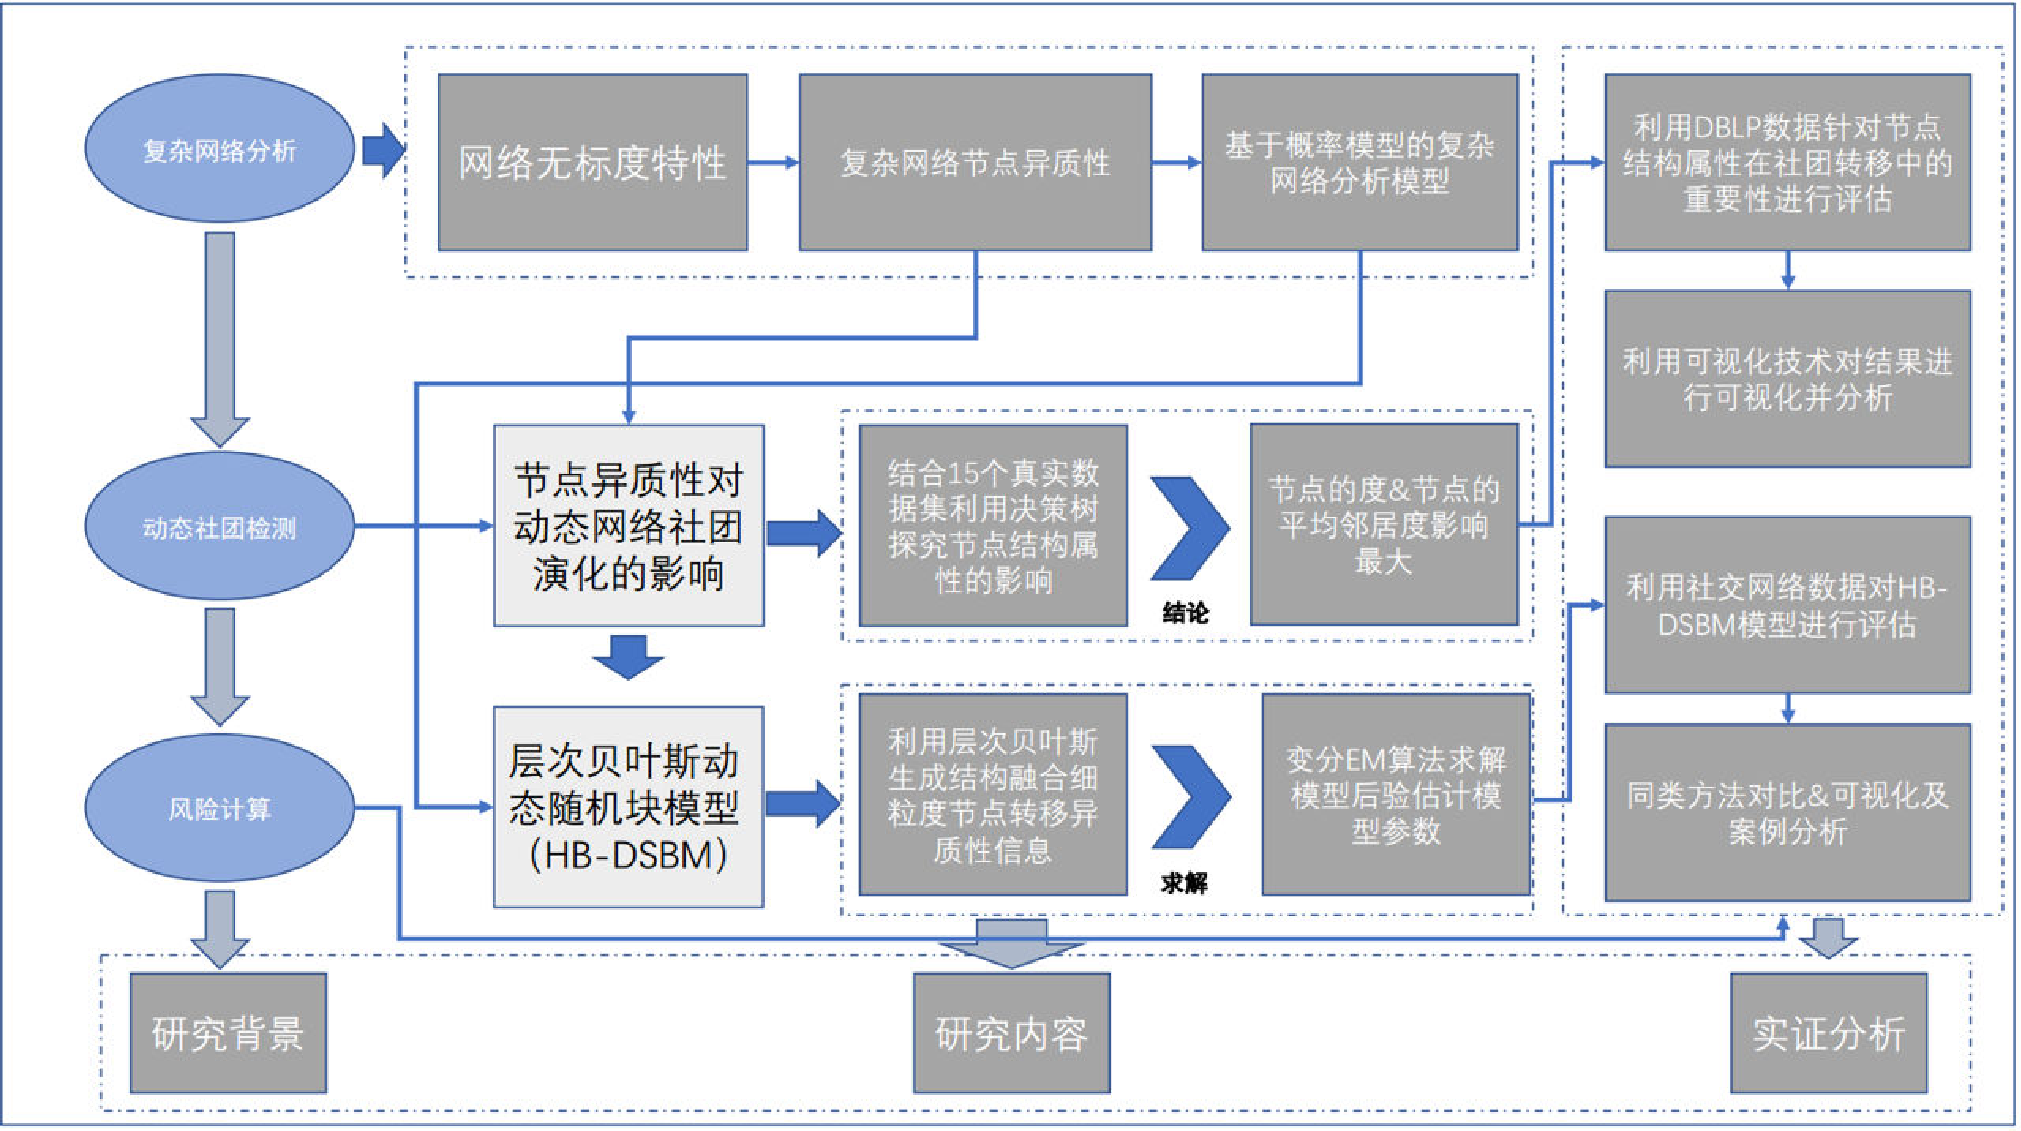
\includegraphics[width = 0.9\textwidth]{./figure/framework1.pdf}
	\caption{研究框架图}
	\label{fig.1}
\end{figure}
以上方法均重点关注动态网络社团检测的精度以及效率,而对于社团演化的关注度并不高。然而社团演化对于动态网络社团检测至关重要,同时社团演化也是一个重要的课题。Yang, Jinfeng~\cite{yang2018structural}等人利用每个社团内的关键节点来匹配相邻社团,进而来把握社团的演化。然而核心节点未必能够代表社团。Gergely Palla~\cite{palla2007quantifying}等人提出社团的出生、消亡、分裂、合并、增长、缩小六种社团行为,被其他研究者广泛借鉴。
社团的演化本质上是由节点之间的连边变化驱动的,因此社团的演化行为与社团内部节点的社团转移之间的关系对于社团演化来说至关重要,然而据我们所知目前还没有对这种关系深入的探究。同时,社团的演化行为也是由社团内的节点的变化而驱动的,目前也没有相关的文献进行详细探究。因此,如图\ref{fig.1}所示,以上两个问题就是本课题将要探究的目标,即探究节点异质性对动态网络社团演化的影响以及利用细粒度演化参数构建动态社团检测模型。
\subsection{城市风险计算现状}
城市风险包含的范围非常广,包括自然灾害城市风险(如地震与台风等)、公共事件类城市风险(如踩踏事件与群体恐慌等)、社会安全城市风险(如核泄漏、恐怖袭击、抢劫枪杀等)、公共卫生安全城市风险(如非典、禽流感与艾滋病等)等。因此对于城市风险来说其风险源广,风险数据量大,其综合识别与整体的管控与治理非常困难。然而针对不同的城市风险需求进行有针对化的计算与治理则难度相对较小,同时其某些特定风险计算需求与网络中的相关算法非常契合,例如网络算法中的关键节点识别就可以用来识别城市风险中的风险点,而风险事件识别则对应了动态网络社团检测。例如社团检测算法可以高效的检测出城市中的不同粒度的团体,再结合社团演化分析就可以检测出不同的事件,通过有效地设置损失函数,就可以对事件风险进行打分并排序,确定不同事件的风险大小。


城市风险计算涉及的数据范围非常广,如城市风险计算包括人类行动轨迹、车辆轨迹、人类电子足迹、社交网络数据、转账数据、城市OD流数据等等,均来自于风险监测模块的多元数据收集。收集后的数据维度广,数据量大,并不能直接进行风险计算,因而需要对数据进行融合,即信息融合。通过多维信息的多层级融合,将数据建模成复杂网络形式数据,进行风险计算。根据不同的风险需求,风险计算可以灵活选择不同的网络算法,如风险因素识别可以利用复杂网络中的关键节点识别算法进行提取,而风险事件则可以利用动态社团检测算法进行计算。

\subsection{主要创新点}

本文的主要创新点包括以下三个方面:

\begin{enumerate}
	\item 发现了动态网络中对节点社团转移影响最大的两个结构属性;
	\item 构建了节点粒度级别演化参数的动态网络社团检测生成模型并为模型求解提出了有效的变分近似算法;
	\item 成功探索了复杂网络社团检测与风险计算的紧密关联并进行了验证。
\end{enumerate}

三个创新点具有紧密的内在关联性,本文通过十五个真实世界复杂网络数据集探索了动态网络中节点的社团转移与节点及社团的结构属性之间的关系,发现了影响节点社团转移的两个结构属性:节点的度以及节点的平均邻居度。这两个结构属性均为节点粒度的结构属性,而社团的属性在节点的社团转移中起到的作用不大,说明节点粒度的社团转移参数在模型中是有必要的。受上述的启发,本文提出了节点粒度的动态网络社团检测模型,并利用变分推断近似求解,使模型适用于真实世界复杂网络。而城市风险计算在城市管理中至关重要,而传统的机器学习算法无法处理具有复杂关联的城市多元数据。依赖于复杂网络及复杂网络社团检测算法,对于城市多元关联性数据,本文提出的算法可以有效的进行处理,同时基于本文算法的处理结果,利用城市风险计算的相关算法可以有效的计算不同事件的风险程度,为城市风险计算与复杂网络社团检测搭建了桥梁。


\section{章节安排}


根据本文的研究框架,文章的章节结构安排如下:

第一章,绪论,介绍复杂网络分析中,社团检测在风险计算中的重要作用以及风险计算的相关流程,研究背景及意义、研究内容框架、主要创新点等。

第二章,相关研究,介绍动态网络社团检测以及风险计算的相关研究,同时介绍本文的统一符号表示等。

第三章,节点结构属性对社团演化影响因素的探究,本文会在真实的网络数据中具体探究动态网络社团检测中,节点的哪些结构属性对社团演化影响较大。

第四章,融合节点级别社团转移参数的动态网络生成模型,本文将会针对经典的动态网络社团检测概率模型-----动态随机块模型,融合更细粒度的演化参数,利用层次贝叶斯生成结构构建对社团演化掌握更准确的新模型:层次贝叶斯动态随机块模型,并在接下来介绍针对层次贝叶斯动态随机块模型的变分推断近似解法。

第五章,案例分析,本章会利用手机信令数据结合动态复杂网络社团检测算法以及风险计算的相关理论知识及算法进行实际的风险计算,验证复杂网络在风险计算中的重要作用。

第六章,总结与展望,本章将总结本课题的工作,并对未来工作进行说明与展望。

